\documentclass{VUMIFPSbakalaurinis}
\usepackage[table]{xcolor}
\usepackage{algorithmicx}
\usepackage{algorithm}
\usepackage{algpseudocode}
\usepackage{amsfonts}
\usepackage{amsmath}
\usepackage{bm}
\usepackage{caption}
\usepackage{color}
\usepackage{float}
\usepackage{graphicx}
\usepackage{listings}
\usepackage{subfig}
\usepackage{wrapfig}
\usepackage{tikz}

\usepackage{enumitem}
\setitemize{noitemsep,topsep=0pt,parsep=0pt,partopsep=0pt}
\setenumerate{noitemsep,topsep=0pt,parsep=0pt,partopsep=0pt}

% Ignore all trivial warnings
\hbadness=5000
% Titulinio aprašas
\university{Vilniaus universitetas}
\faculty{Informatikos institutas}
\department{Programų sistemų katedra}
\papertype{Bakalauro baigiamasis darbas }
\title{Srautinio apdorojimo modulių generavimas kintant rodiklių duomenų struktūrai}
\titleineng{Generation of Stream Processing Modules upon Change of Indicator Data Structure}
\author{Vytautas Žilinas}
\supervisor{lekt. Andrius Adamonis}
\reviewer{assoc. prof., dr. Karolis Petrauskas}
\date{Vilnius – \the\year}

% Nustatymai
% \setmainfont{Palemonas}   % Pakeisti teksto šriftą į Palemonas (turi būti įdiegtas sistemoje)
\bibliography{bibliografija}

\begin{document} 
\maketitle

\cleardoublepage\pagenumbering{arabic}
\setcounter{page}{2}

\sectionnonumnocontent{Santrauka}
Šį darbą sudaro teorinė ir eksperimentinė dalis. Teorinėje dalyje apibrėžiamas rodiklis, jo struktūra ir struktūros pokyčiai. Apibrėžiami kokie yra įmanomi pokyčiai ir kaip eksperimentinėje dalyje kuriamas sprendimas prie pokyčių prisitaikys. Specifikuojama duomenų struktūra ir duomenų struktūrų apjungimo ir skirtumo operacijas. Apibrėžiamas srautinis apdorojimas ir pasirenkama sistema, kuri bus naudojama eksperimentinėje dalyje. Remiantis gautais rezultatais
nustatoma, kad šiam uždaviniui spręsti pasirenkama "Heron" srautinio apdorojimo sistema. Remiantis pasirinkta srautinio apdorojimo sistema ir apibrėžta rodiklių duomenų struktūra, eksperimentui nusprendžiama generuoti srautinio apdorojimo modulius parašytus "Python" programavimo kalba. Eksperimentinėje dalyje remiantis pasiūlytu modeliu realizuojama bandomoji sistemos versija. Atliekant skirtingų kiekių rodiklių duomenų ir rodiklių duomenų pokyčių simuliaciją stebėjimais analizuojamas šios sistemos tinkamumas apibrėžtam uždaviniui spręsti. Gauti tyrimų rezultatai lyginami, pateikiamos išvados. Taip įrodoma, kad toks sprendimas gali būti įgyvendinamas ir kad kodo generavimas ir srautinio apdorojimo sistema "Heron" yra tinkamas sprendimas kintančių rodiklių uždaviniui spręsti.
\raktiniaizodziai{srautinis apdorojimas, kodo generavimas, rodikli, rodiklio duomens pokyčiai}   

\sectionnonumnocontent{Summary}
This work consists of a theoretical and an experimental part. Theoretical part defines the indicator, its structure and changes in indicator structure. It define what changes are possible and how the developed solution in the experimental part will adapt to the changes, specifies the data structure and data structure merging and difference operations, defines stream processing and selects the system to be used in the experimental part. Based on the results
it is determined that "Heron" stream processing system is chosen to solve this task. Based on the selected stream processing system and the defined data structure of indicator, it is decided to generate streaming modules written in "Python" programing language. In the experimental part, a pilot version of the system is implemented based on the proposed model. By doing the simulation using varying amounts of indicators and indicator changed, the suitability of this system for a defined task is tested. The results of this research are compared and conclusions are given. This demonstrates that such a solution can be implemented and that the code generation and streaming system "Heron" is the right solution to deal with the challenge of changing indicators.
\keywords{stream processing, code generation, indicator, indactor structure change}

\tableofcontents

\sectionnonum{Įvadas}
 
% TODO: Įžangoje apžvelgti srautinį apdorojimą ir kodo generavimą.
Šiame darbe yra nagrinėjamas rodiklių duomenų apdorojimas ir kuriamas sprendimas galintis prisitaikyti prie kintančių rodiklių duomenų struktūros. Rodiklių duomenimis vadiname duomenis, aprašančius kažkokių objektų savybes arba veiklos procesų rezultatus. Šiuos duomenis galima transformuoti, analizuoti ir grupuoti pagal pasirinktus rodiklius, pavyzdžiui: bazinė mėnesinė alga, mirusiųjų skaičius pagal mirties priežastis, krituliai per metus. Taip pat rodiklių struktūra gali keistis laikui bėgant: objektų atributų taksonomija (pvz. mirties priežasčių sąrašas, finansinių sąskaitų sąrašas) arba įrašo atributų sąrašai. Surenkamu rodiklių duomenų kiekis visada didėja, taip pat ir duomenų kiekis, kuriuos reikia apdoroti pagal rodiklius auga, todėl standartiniai sprendimai, pavyzdžiui reliacinės duomenų bazės netinka dėl ilgos apdorojimo trukmės. Rodiklių duomenų bazės pasižymi tuo, kad duomenys į jas patenka iš daug skirtingų tiekėjų ir patekimo laikas tarp tiekėjų nėra sinchronizuojamas, o suagreguotą informaciją vartotojai gali užklausti bet kurio metu. Todėl šiame darbe bus nagrinėjamas srautinis duomenų apdorojimas, kuris patenkančius duomenis apdoros realiu laiku, ir saugos jau apdorotus.  \par
Realaus laiko duomenų apdorojimas (angl. Real-time data processing) yra jau senai nagrinėjamas, kaip būdas apdoroti didelių kiekių duomenis (angl. Big data). Vienas iš realaus laiko apdorojimo sprendimų yra srautinis duomenų apdorojimas \cite{BigData, StreamProcessingInData}. Srautinis duomenų apdorojimas (angl. stream processing) – programavimo paradigma, kuri yra ekvivalenti duomenų srauto programavimo (angl. dataflow programming) paradigmai \cite{shortstreamproc}. 
Duomenų tėkmės programavimo paradigmos idėja yra, kad programa susidaro iš skirtingu modulių, kurie nepriklauso vienas nuo kito, ir tai leidžia sukonstruoti paraleliai skaičiuojančias programas. 
Vienas iš pirmųjų duomenų tėkmės programavimo kompiliatorių yra BLODI - blokų diagramų kompiliatorius (angl. BLOck DIagram compiler), su kuriuo buvo kompiliuojamos BLODI programavimo kalba parašytos programos \cite{kelly1961block}.  Šia kalba parašytos programos atitinka inžinerinę elektros grandinės schemą, kur duomenys keliauja per komponentus kaip ir elektros grandinėje. Pasinaudojant šiai programavimo paradigmai sukurtai sistemai bus sukurtas sprendimas, kuris generuos modelius, kurie galės apdoroti rodiklių duomenis ir talpins jau apdorotus duomenis kitoje talpykloje \cite{8Requirements}. 
\par
Kadangi rodiklių yra daug skirtingų ir jie laikui bėgant gali kisti reikia, kad sprendimas kuris juos apdoros galės prisitaikyti prie poreikiu. Yra keli būdai kaip tai galima išspręsti:
\begin{itemize}
    \item Rankinio atnaujinimo sprendimas. Sukuriamas sprendimas pagal esamus reikalavimus ir išskiriamas žmogus, kuris pagal naujus poreikius gali sukurti naujas arba pakeisti esamas apdorojimo programas. 
    \item Universalus sprendimas. Sukuriamas srautinio duomenų apdorojimo sprendimas, kuris apdoroja visus duomenis pagal visus įmanomus rodiklius.
    \item Kodo generavimo sprendimas. Sukuriamas sprendimas, kuris generuoja srautinio duomenų apdorojimo programas pagal iš anksto aprašytą struktūrą.  
\end{itemize}   
Šie sprendimai turi būti pritaikyti pagal sprendžiama problemą. Jei nėra numatomas kitimas pagal ką turi būti apdorojami duomenis, tai galima pasirinkti ir rankinio apdorojimo sprendimą, kadangi nėra didelės tikimybės, kad teks keisti sprendimą. Toks sprendimas tiktų apdorojant išmaniųjų skaitiklių duomenis \cite{skaitikliai}. Universalus sprendimas taip pat gali būti tinkamas jei įeinantis duomenis yra specifiški ir yra poreikis juos visus apdoroti. Toks sprendimas gali būti aktualus apdorojant duomenis iš sensorių, kurie matuoja namų būsena (temperatūra, drėgmę ir t.t.) ir bet koks naujas sensorius taip pat turi būti prijungtas ir apdorotas \cite{yang2017iot}. Šiame darbe buvo pasirinkta naudoti kodo generavimą siekiant sukurti sprendimą tinkanti bendram atvejui, kai duomenis yra nekonkretus ir ne visi reikalingi ir rodikliai kinta dažnai siekiant išgauti kuo daugiau informacijos iš įeinančių duomenų. \par
Kodo generavimas - todo \par
Darbe bus nagrinėjamas sprendimas generuojantis srautinio apdorojimo modulius pagal ateinančius rodiklių duomenis. 
Kadangi rodikliai yra  
Šiame darbe kuriamas sprendimas yra aktualus, kai kinta duomenų struktūra ir norėtume šis sprendimas prisitaiko 
prie duomenų pokyčių kurdamas naujus apdorojimo modulius.


Tikslas: Sukurti rodiklių duomenų srautinio apdorojimo platformos architektūrą, kuri, naudojant kodo generavimą, dinamiškai prisitaiko prie rodiklių duomenų struktūrų pokyčių.

Uždaviniai:
\begin{enumerate}
    \item Apibrėžti rodiklių duomenų modelį ir galimus rodiklių duomenų struktūros pokyčius.
    \item Apibrėžti, kaip specifikuoti duomenų struktūrą ir duomenų struktūrų versijų specifikacijų apjungimo ir skirtumo operacijas.
    \item Atlikus šaltinių analizę pasirinkti srautinio duomenų apdorojimo sistemą, joje sukurti sudarytos architektūros sprendimą ir atlikti bandymus.
\end{enumerate}

\section{Rodiklių duomenys}

Rodiklių duomenys - tai duomenis, kurie apibrėžia bet kokius duomenis, kuriuos galime grupuoti pagal tam kitus elementus. Rodiklį sudaro pirminis raktas, kuris susideda iš vieno arba daug duomenų ir reikšmių sąrašas, kurį galime grupuoti pagal apibrėžtą raktą.      
Rodiklių duomenų gali būti daug todėl reikia bendro modelio, kuris gali apibrėžti visus įmanomus rodiklius. 
\subsection{Rodiklių duomenų modelis}

Darbo tikslui išpildyti buvo sukurtas modelis, kurio pagalba galime apibrėžti rodiklį. Pagal šį apibrėžimą bus generuojama srautinio apdorojimo architektūra.

\begin{figure}[H]
    \centering
    \includegraphics[width=1\textwidth]{img/rodiklis.jpg}
    \caption{Rodiklis}
    \label{img:rodiklis}
\end{figure}

Šiame darbe šis rodiklis bus užrašomas skaidant į dvi dalis: \\
Raktas ir apribojimai:
\[ [\text{Raktas 1, Raktas N}]
    \>\> ; \>\>  
    \begin{array}{|c|c|}
        \hline
        \text{Apribojimas 1} & \text{Apribojimas N} \\ 
        \hline
        \text{Reikšmė 1} & \text{Reikšmė N} \\ 
        \text{Operatorius 1} & \text{Operatorius N} \\
        \text{Riba 1} & \text{Riba N} \\
        \hline 
   \end{array}
\]
Reikšmės: \\
\[
    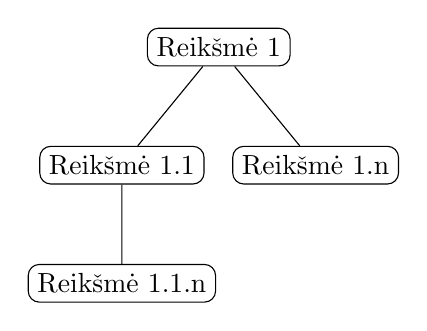
\begin{tikzpicture}[sibling distance=7em,
        every node/.style = {shape=rectangle, rounded corners,
                             draw, align=center,
                             top color=white, bottom color=white}]
        \node {Reikšmė 1}
                child { node {Reikšmė 1.1} 
                    child { node { Reikšmė 1.1.n} } }
                child { node {Reikšmė 1.n} } ;
    \end{tikzpicture} 
    \>\>\>\>\>\>\>\>
    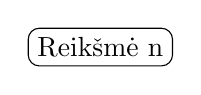
\begin{tikzpicture}[sibling distance=10em,
        every node/.style = {shape=rectangle, rounded corners,
            draw, align=center,
            top color=white, bottom color=white}]]
        \node {Reikšmė n} ;
    \end{tikzpicture}  
\]
\section{Rodiklių duomenų pokyčiai}

Kadangi einant laiku duomenis gali keistis ir atitinkamai gali keistis ir rodiklių duomenų tipas, kuriuos reikia surinkti. Tarkime mes turime rodiklį, kuris apibrėžia žmogaus, kuris dirba pagal terminuotą darbo sutartį, metines pajamas, kurios susideda iš gaunamo atlyginimo ir premijų:
Raktas ir apribojimai:
\[ [\text{Žmogus, Metai}]
    \>\> ; \>\>  
    \begin{array}{|c|}
        \hline
        \text{Terminuotą darbo sutartis}  \\ 
        \hline
        \text{Darbo sutarties tipas} \\ 
        \text{LYGU}  \\
        \text{TERMINUOTA} \\
        \hline 
   \end{array}
\]
Reikšmės: \\
\[
    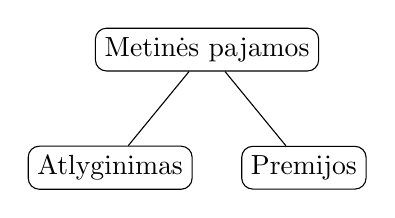
\begin{tikzpicture}[sibling distance=7em,
        every node/.style = {shape=rectangle, rounded corners,
                             draw, align=center,
                             top color=white, bottom color=white}]
        \node {Metinės pajamos}
                child { node {Atlyginimas} }
                child { node {Premijos} } ;
    \end{tikzpicture} 
\]
Pavyzdžiui, jei atsiranda poreikis fiksuoti, ne tik iš gaunama atlygimą ir premiją, bet ir iš loterijose laimėtus pinigus. Taip pat tarkime, jog terminuota darbo sutartis buvo išskaidyta į terminuotą darbo sutartį ir laikinojo darbo sutartį ir mums reikia įtraukti duomenis pagal abu apribojimus. Mūsų rodiklis, turėtų atsinaujinti atitinkamai:

Raktas ir apribojimai:
\[ [\text{Žmogus, Metai}]
    \>\> ; \>\>  
    \begin{array}{|c|c|}
        \hline
        \text{Terminuotą darbo sutartis} & \text{Laikinojo darbo sutartis} \\ 
        \hline
        \text{Darbo sutarties tipas} & \text{Darbo sutarties tipas} \\ 
        \text{LYGU} & \text{LYGU} \\
        \text{TERMINUOTA} & \text{LAIKINOJI} \\
        \hline 
   \end{array}
\]
Reikšmės: \\
\[
    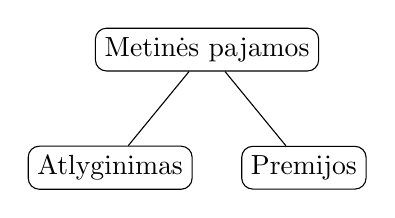
\begin{tikzpicture}[sibling distance=7em,
        every node/.style = {shape=rectangle, rounded corners,
                             draw, align=center,
                             top color=white, bottom color=white}]
        \node {Metinės pajamos}
            child { node {Atlyginimas} }
            child { node {Premijos} } ;
    \end{tikzpicture} 
    \>\>\>\>\>\>\>\>
    \begin{tikzpicture}[sibling distance=10em,
        every node/.style = {shape=rectangle, rounded corners,
            draw, align=center,
            top color=white, bottom color=white}]]
        \node {Loterijų laimėjimai} ;
    \end{tikzpicture}  
\]

\subsection{Galimi pokyčiai}

\subsubsection{Pirminis raktas}
Mes savo rodiklyje pakeitėme apribojimus ir reikšmes, tačiau nekeitėme pirminio rakto todėl, kad tokiu atveju grupavimas nebeturėtų prasmės. Tarkime, kad norime nuo 2019 metų rinkti duomenis ne metinius, o kas mėnesį. Tokiu atveju jau surinkti duomenis nebeturi prasmės, nes bandoma lyginti metinius rezultatus su mėnesiais. Jei tai toks elementas, kuris gali kisti ir nėra renkama reikšmė tai turėtų būti apibrėžiama kaip apribojimas. Jei yra poreikis keisti pirminį raktą, reikia kurti naują rodiklį ir, jei yra poreikis pagal jį suagreguoti naujus ir istorinius duomenis, turi būti iš naujo apdoroti visi turimi duomenys.     

\subsubsection{Apribojimai}

\subsubsection{Reikšmės}

\section{Srautinio duomenų apdorojimo sprendimų analizė}

\subsection{Srautinis duomenų apdorojimas} \label{strprocess}

Siekiant apžvelgti modernias srautinio duomenų apdorojimo architektūras reikia apsibrėžti srautinio apdorojimo sistemų galimybes.
2005 metais Michael Stonebraker apibrėžė 8 taisykles realaus laiko (angl. real-time) srautinio duomenų apdorojimo architektūrai \cite{stonebraker20058}:
\begin{enumerate}[label=\arabic*]
    \item taisyklė: Duomenys turi judėti. Žemo uždelstumo užtikrinimui sistema turi apdoroti duomenis nenaudojant duomenų saugojimo operacijų. 
    Taip pat sistema turi ne pati užklausti duomenų, o gauti juos iš kito šaltinio asinchroniškai. 
    \item taisyklė: Duomenų transformacijos turi būti vykdomas SQL pobūdžio užklausomis. Žemo abstrakcijos lygmens srautinio apdorojimo sistemos reikalauja ilgesnio 
    programavimo laiko ir brangesnio palaikymo. Tuo tarpu aukšto abstrakcijos lygmens sistema 
    naudojanti SQL užklausas, kurias žino dauguma programuotojų ir yra naudojamos daugelyje skirtingų sistemų, leidžia efektyviau kurti srautinio apdorojimo sprendimus.
    \item taisyklė: Architektūra turi susidoroti su duomenų netobulumais. Architektūra turi palaikyti galimybę nutraukti individualius skaičiavimus
    tam, kad neatsirastų blokuojančių operacijų, kurios sustabdo vieno modulio veikimą ir tuo pačiu visos architektūros veikimą. Taip pat ši 
    architektūra turi sugebėti susidoroti su vėluojančiomis žinutėmis, pratęsiant laiko tarpą, per kurį ta žinutė turi ateiti.
    \item taisyklė: Architektūra turi būti deterministinė. Kiekvieną kartą apdorojant tuos pačius duomenis rezultatai turi būti gaunami tokie patys.
    \item taisyklė: Architektūra turi gebėti apdoroti išsaugotus duomenis ir realiu laiku gaunamus duomenis. Sistema parašyta su tokia architektūra turi galėti apdoroti jau esančius duomenis taip pat kaip ir 
    naujai ateinančius. Toks reikalavimas buvo aprašytas, nes atsirado poreikis nepastebimai perjungti apdorojimą iš istorinių duomenų į realiu laiku ateinančius duomenis automatiškai.
    \item taisyklė: Architektūra turi užtikrinti duomenų saugumą ir apdorojimo prieinamumą. Kadangi sistema turi apdoroti didelius kiekius duomenų, architektūra klaidos atveju, turi sugebėti persijungti į atsarginę
    sistemą ir tęsti darbą toliau. Taip pat tokios klaidos atveju atsarginė sistema turi būti apdorojusi visus duomenis ir sugebėti iš karto priimti naujus duomenis, o ne apdoroti duomenis iš pradžių.
    \item taisyklė: Architektūra turi užtikrinti sugebėjimą paskirstyti sistemos darbus automatiškai. Srautinio apdorojimo sistemos turi palaikyti kelių procesoriaus gijų operacijas. Taip pat sistema turi galėti 
    veikti ant kelių kompiuterių vienu metu ir prireikus paskirstyti resursus pagal galimybes.
    \item taisyklė: Architektūra turi apdoroti ir atsakyti akimirksniu. Anksčiau minėtos taisyklės nėra svarbios, jeigu sistema nesugeba greitai susidoroti su dideliu kiekiu naujų duomenų. 
    Todėl turi būti naudojamas ne tik teisingas ir greitas srautinio apdorojimo sprendimas, bet ir gerai optimizuota sistema.
\end{enumerate}\par 
Šie reikalavimai yra sukurti tik teoriškai ir srautinio apdorojimo sprendimai neprivalo jų įgyvendinti \cite{stonebraker20058}. 
Todėl norint sužinoti tam tikro srautinio duomenų apdorojimo sprendimo tinkamumą uždaviniui reikia išanalizuoti to sprendimo galimybes.   

\subsection{Srautinio duomenų apdorojimo sistemos}

Šiame skyriuje lyginamos trys atviro kodo srautinio apdorojimo sprendimai "Apache Storm", "Apache Spark" ir "Apache Flink" ir "Heron" pagal:
\begin{itemize}
    \item Pristatymo semantika (angl. delivery semantics) - apibrėžia pagal kokį modelį bus pristatyti duomenys. Egzistuoja trys semantikos \cite{ensar20}: 
    \begin{itemize}
        \item Bent vieną kartą (angl. at-least-once) užtikrina, kad duomenys bus apdoroti bent kartą, bet gali atsirasti dublikatų. 
        \item Ne daugiau vieno karto (angl. at-most-once) užtikrina, kad duomenys bus apdoroti daugiausiai tik vieną kartą, bet gali atsirasti praradimų. 
        \item Tiksliai vieną kartą (angl. exactly-once) užtikrina, kad duomenys bus apdoroti tik vieną kartą net ir atsiradus klaidoms.
    \end{itemize}
    \item Uždelstumas (angl. latency) - apibrėžia laikų sumą - kiek laiko trūko viena operacija ir kiek laiko ši operacija turėjo laukti eilėje kol bus pabaigtos kitos operacijos \cite{karimov2018benchmarking}.
    \item Pralaidumas (angl. throughput) - apibrėžia kiek pavyks įvykdyti operacijų per tam tikrą laiko tarpą.
    \item Abstrakcijos lygmuo (angl. abstraction) - apibrėžia kokio lygmens programavimo sąsają pateikia sprendimas.
\end{itemize}

\subsection{Pristatymo semantika}
"Apache Spark" ir "Apache Flink" sprendimų pristatymo semantika yra tiksliai vieną kartą (angl. exactly-once), tai reiškia, kad visi duomenys bus apdoroti tik vieną kartą. Tačiau tam, kad užtikrinti šią semantiką sprendimas sunaudoja daug resursų, nes reikia užtikrinti, kad operacija bus vykdoma būtent vieną kartą kiekviename srautinio apdorojimo žingsnyje: duomenų gavime, kuris stipriai priklauso nuo duomenų šaltinio, duomenų transformacijos, kuria turi užtikrinti pats srautinio apdorojimo sprendimas, ir duomenų saugojime, tai turi būti užtikrinta sprendimo ir naudojamos saugyklos \cite{zhang20}.\par

"Apache Storm" pristatymo semantika yra bent vieną kartą (angl. at-least-once), tai reiškia, kad į šį sprendimą siunčiami duomenys bus visada apdoroti, tačiau kartais gali būti apdoroti kelis kartus \cite{prithi20}. Jeigu sprendimas reikalauja tiksliai vieno karto apdorojimo, tada turi būti pasirinkti "Apache Spark", "Apache Flink" sprendimai arba "Heron" - "Apache Storm" sprendimu paremtas sprendimas galintis nurodyti pristatymo semantika. Tačiau jei uždavinys nereikalauja tiksliai vieno karto apdorojimo, tai geriau rinktis bent vieną kartą ar ne daugiau vieno karto semantikas, kadangi jos neturi papildomų apsaugų, kurios reikalingos tiksliai vieno karto apdorojimui, ir todėl veikia greičiau \cite{zhang20}. \par

"Heron" sprendimų pristatymo semantika gali būti keičiama, programuotojas kurdamas srautinio apdorojimo programą aprašo kokio tipo pristatymo semantikos jam reikia \cite{delivery-semantics}. Todėl šis sprendimas yra universaliausias iš visų ir tinka jei kuriamas sprendimas turi būti dinamiškas ir kuo išsamiau konfigūruojamas.   

\subsection{Uždelstumas}

Uždelstumas srautinio apdorojimo sprendimams yra matuojamas laiku, kuris parodo kaip greitai sprendimas įvykdo vieną operaciją, nuo jos patekimo į eilę iki šios operacijos apdorojimo pabaigos. Pagal \cite{Lopez2016APC} aprašytus Martin Andreoni Lopez "Apache Storm", "Apache Spark" ir "Apache Flink" bandymus galima matyti, kad būtent "Apache Storm" turi mažiausią uždelstumą. Kadangi parinkus tinkamą paralelizmo parametrą šis sprendimas su užduotimi susidorojo net iki 15 kartų greičiau. Antroje vietoje liko "Apache Flink", o po jos "Apache Spark". \par

Tačiau "Heron" sprendimas yra sukurtas siekiant pagerinti "Apache Storm" sprendimo greitaveika ir suteikti lengvą būdą pereiti nuo "Apache Storm" API prie "Heron", todėl jo uždelstumas yra dar mažesnis negu "Apache Storm" \cite{Kulkarni:2015:THS:2723372.2742788}.

\subsection{Pralaidumas}

Pralaidumas apibrėžia kokį kiekį procesų sistema gali įvykdyti per tam tikrą laiko tarpą. 2016 metais Sanket Chintapalli \cite{chintapalli2016benchmarking} išmatavo "Apache Storm", "Apache Spark" ir "Apache Flink" sprendimų pralaidumą ir uždelstumą bei palygino rezultatus. Kaip ir anksčiau manyta, "Apache Spark" turėjo aukščiausia pralaidumą iš visų, kadangi jis vienintelis duomenis apdoroja mikro-paketais. Antroje vietoje liko "Apache Flink", kuris yra subalansuotas
pralaidumo atveju ir paskutinis liko "Apache Storm", kuris turi žemą uždelstumą, todėl nukenčia pralaidumas. "Heron" tuo tarpu turi aukštesnį pralaidumą ir žemesnį uždelstumą nei "Apache Storm" \cite{TwitterHeron}. 

\subsection{Abstrakcijos lygmuo}

"Apache Storm" parašytos programos yra žemo abstrakcijos lygmens, tai reiškia, kad turi būti aprašyti visi srautinio apdorojimo moduliai: 
setSpouts(..), kuriame nustatoma duomenų įeiga ir koks bus paralelizmo lygis, setBolt(..), kuriame nustatomi apdorojimo moduliai, kokius duomenis gaus iš prieš tai buvusio modulio ir paralelizmo lygis. Kiekvieno modulio execute() metodas aprašo, kaip šis modulis turi apdoroti duomenis \cite{tutpoint}. Šio sprendimo programų kūrimo laikas užtruks ilgiau negu kitiems sprendimams su aukštu abstrakcijos lygmeniu, tačiau žemas abstrakcijos leidžia rašyti daug greičiau veikiančias programas, kadangi programuotojas turi pilną kontrolę. \par

"Apache Spark" parašytos programos yra aukšto abstrakcijos lygmens. Programa aprašoma funkciškai, todėl kodo rašymas trunka daug trumpiau ir jį yra daug patogiau skaityti. Tačiau prarandama galimybė optimizuoti ir paralelizmo klausimas paliekamas sprendimui. Kadangi "Apache Spark" yra ne pilnai srautinis, o mikro-paketinis (angl. micro-batching) sprendimas, todėl vartotojas turi apsirašyti kokio dydžio paketais bus renkami duomenys \cite{shoro2015big}. \par

"Apache Flink" parašytos programos yra aukšto abstrakcijos lygmens. "Apache Flink" sprendimas pati užsiima resursų distribucija, todėl programuotojui lieka tik parašyti veikianti kodą, o sistema pati susitvarkys su paralelizmu \cite{flinkdoc}. Tačiau tai reiškia, kad su šiuo sprendimu parašytos programos nepavyks optimizuoti taip pat gerai kaip žemo abstrakcijos lygmens sprendimai. \par

"Heron" sprendimas turi skirtingus API, kurie naudoja skirtingus abstrakcijos lygius, kuriuos galima rinktis pagal tinkamumą sprendžiamai problemai. Darbo rašymo metu "Heron" turi 4 skirtingus API:
\begin{itemize}
    \item "Heron Streamlet API" - aukšto abstrakcijos lygmens API, rašomas su "Java" programavimo kalba. Panaši sintaksė į "Apache Flink" rašomų sprendimų.
    \item "Heron ECO API" - eksperimentinis aukšto abstrakcijos lygmens API, rašomas su "Java" programavimo kalba. Skiriasi nuo "Heron Streamlet API", nes modulių apdorojimo eiliškumas apsirašo YAML formatų, kas leidžia keisti sukurtos srautinio duomenų apdorojimo programos struktūrą nekeičiant kodo.
    \item "Heron Topology API for Java" - žemo abstrakcijos lygmens API, rašomas su "Java" programavimo kalba. Rašomas identiškas kodas, kaip ir "Apache Storm", kadangi "Heron" sprendimas buvo sukurtas siekiant pagerinti "Apache Storm".
    \item "Heron Topology API for Python" - žemo abstrakcijos lygmens API, rašomas su "Python" programavimo kalba. Su šiuo API kuriami srautinio apdorojimo sprendimai yra panašus į "Apache Storm", tik su "Python" programavimo kalbos privalumais.
\end{itemize}  


\subsection{Apibendrinimas}
Iš šių keturių sprendimų reikėjo pasirinkti vieną, kuri labiausiai tiks rodiklių duomenų apdorojimui. Šis sprendimas turi sugebėti greitai apdoroti duomenis, prioretizuojant greitį virš tikslumo, kadangi vienas iš pagrindinių naudotojų yra statistiką renkančios įstaigos, kurios gali sau leisti tam tikrą paklaidą, ir programuotojas turi galėti aprašyti daug skirtingų sprendimų skirtingiems rodikliams.\par

\begin{table}[!htbp]
    \begin{center}
        \caption{Srautinių duomenų apdorojimo sprendimų palyginimas}
        \label{table:comparer}
        \begin{tabular}{ | l | c | c | c | c | } 
            \hline
            \cellcolor[gray]{0.8} Charakteristika & \cellcolor[gray]{0.9} "Apache Storm" & \cellcolor[gray]{0.9} "Apache Spark" & \cellcolor[gray]{0.9} "Apache Flink" & \cellcolor[gray]{0.9} "Heron" \\* \hline
            \cellcolor[gray]{0.9} Pristatymas & Bent vieną kartą & Tiksliai vieną kartą & Tiksliai vieną kartą & Pasirinktinai \\* \hline
            \cellcolor[gray]{0.9} Uždelstumas & Žemas & Aukštas & Vidutinis & Žemas \\* \hline
            \cellcolor[gray]{0.9} Pralaidumas & Žemas & Aukštas & Vidutinis & Vidutinis \\* \hline
            \cellcolor[gray]{0.9} Abstrakcija & Žemas & Aukštas & Aukštas & Pasirinktinai \\* \hline
        \end{tabular}
    \end{center}
\end{table}\par

Pagal atlikta analizę \ref{table:comparer} lentelėje ir apsibrėžtų reikalavimų šiam uždaviniui tinkamiausias srautinio apdorojimo sprendimas yra "Heron". \par
Čia parašyti apie pasirinkimo semantikas \par
Čia parašyti apie abstrakcija \par
Čia parašyti apie Python \par
 

\section{Eksperimentas}


\sectionnonum{Rezultatai}

\begin{enumerate}
    \item Apibrėžta rodiklių duomenų struktūra ir galimi duomenų struktūros pokyčiai.
    \item Pasirinktai srautinio duomenų apdorojimo sistemai sukurto sprendimo atliktų eksperimentų rezultatai - generuojamas kodas ir jo savybes. 
\end{enumerate}

\sectionnonum{Išvados}
Rezultatų ir išvadų dalyje išdėstomi pagrindiniai darbo rezultatai (kažkas
išanalizuota, kažkas sukurta, kažkas įdiegta), toliau pateikiamos išvados
(daromi nagrinėtų problemų sprendimo metodų palyginimai, siūlomos
rekomendacijos, akcentuojamos naujovės). Rezultatai ir išvados pateikiami
sunumeruotų (gali būti hierarchiniai) sąrašų pavidalu. Darbo rezultatai turi
atitikti darbo tikslą.

\printbibliography[heading=bibintoc] 


\appendix 


\end{document}
